\documentclass[12pt, letterpaper, preprint, comicneue]{aastex63}
%\usepackage[default]{comicneue} % comic sans font for editing
\usepackage[T1]{fontenc}
\input{vc}
\usepackage{color}
\usepackage{amsmath}
\usepackage{natbib}
\usepackage{ctable}
\usepackage{bm}
\usepackage[normalem]{ulem} % Added by MS for \sout -> not required for final version
\usepackage{xspace}
\usepackage{csvsimple} 

\usepackage{graphicx}
\usepackage{pgfkeys, pgfsys, pgfcalendar}


% typesetting shih
\linespread{1.08} % close to 10/13 spacing
\setlength{\parindent}{1.08\baselineskip} % Bringhurst
\setlength{\parskip}{0ex}
\let\oldbibliography\thebibliography % killin' me.
\renewcommand{\thebibliography}[1]{%
  \oldbibliography{#1}%
  \setlength{\itemsep}{0pt}%
  \setlength{\parsep}{0pt}%
  \setlength{\parskip}{0pt}%
  \setlength{\bibsep}{0ex}
  \raggedright
}
\setlength{\footnotesep}{0ex} % seriously?

% citation alias

% math shih
\newcommand{\setof}[1]{\left\{{#1}\right\}}
\newcommand{\given}{\,|\,}
\newcommand{\lss}{{\small{LSS}}\xspace}

\newcommand{\Om}{\Omega_{\rm m}} 
\newcommand{\Ob}{\Omega_{\rm b}} 
\newcommand{\OL}{\Omega_\Lambda}
\newcommand{\smnu}{M_\nu}
\newcommand{\sig}{\sigma_8} 
\newcommand{\mmin}{M_{\rm min}}
\newcommand{\BOk}{\widehat{B}_0} 
\newcommand{\hmpc}{\,h/\mathrm{Mpc}}
\newcommand{\bfi}[1]{\textbf{\textit{#1}}}
\newcommand{\parti}[1]{\frac{\partial #1}{\partial \theta_i}}
\newcommand{\partj}[1]{\frac{\partial #1}{\partial \theta_j}}
\newcommand{\mpc}{{\rm Mpc}}
\newcommand{\eg}{\emph{e.g.}}
\newcommand{\ie}{\emph{i.e.}}

% cmds for this paper 
\newcommand{\gr}{g{-}r}
\newcommand{\fnuv}{FUV{-}NUV}
\newcommand{\sfr}{{\rm SFR}}
\newcommand{\ssfr}{{\rm SSFR}}
\newcommand{\mtaum}{m_{\tau,M_*}}
\newcommand{\mtaus}{m_{\tau,{\rm SSFR}}}
\newcommand{\ctau}{c_\tau}
\newcommand{\mdeltam}{m_{\delta,M_*}}
\newcommand{\mdeltas}{m_{\delta,{\rm SFR}}}
\newcommand{\cdelta}{c_\delta}
\newcommand{\eda}{EDA}


\newcommand{\specialcell}[2][c]{%
  \begin{tabular}[#1]{@{}c@{}}#2\end{tabular}}
% text shih
\newcommand{\foreign}[1]{\textsl{#1}}
\newcommand{\etal}{\foreign{et~al.}}
\newcommand{\opcit}{\foreign{Op.~cit.}}
\newcommand{\documentname}{\textsl{Article}}
\newcommand{\equationname}{equation}
\newcommand{\bitem}{\begin{itemize}}
\newcommand{\eitem}{\end{itemize}}
\newcommand{\beq}{\begin{equation}}
\newcommand{\eeq}{\end{equation}}

%% collaborating
\newcommand{\todo}[1]{\marginpar{\color{red}TODO}{\color{red}#1}}
\definecolor{orange}{rgb}{1,0.5,0}
\newcommand{\ch}[1]{{\color{orange}{\bf CH:} #1}}

\begin{document} \sloppy\sloppypar\frenchspacing 

\title{Cosmology with Only the Photometry of Many Galaxies} 
\date{\texttt{DRAFT~---~\githash~---~\gitdate~---~NOT READY FOR DISTRIBUTION}}

\newcounter{affilcounter}
\author{ChangHoon Hahn}
\altaffiliation{changhoon.hahn@princeton.edu}
\affil{Department of Astrophysical Sciences, Princeton University, Peyton Hall, Princeton NJ 08544, USA} 

\author{Francisco Villaescusa-Navarro}

\begin{abstract}
    We present the first cosmological constraints from photometric observations
    of galaxies. 
    Villaescusa-Navarro+(2022) recently demonstrated that a galaxy's internal
    physical properties contain a significant amount of cosmological
    information: *i.e.* cosmology with one galaxy. These physical properties,
    however, cannot be directly measured from observations. In this talk, I
    will present how we can go beyond theoretical demonstrations to infer
    cosmological constraints from actual galaxy observables (*e.g.* optical
    SDSS photometry) using simulation-based inference and neural density
    estimation on the CAMELS dataset. While the cosmological information from
    photometric observations of a single galaxy is limited, I will present
    preliminary results that place significant cosmological constraints from
    hierarchical population inference of photometry from thousands of SDSS
    galaxies. Furthermore, I will discuss domain adaptation (TNG versus SIMBA)
    and challenges in SED modeling, which underpins the connection between the
    simulations and observations. Lastly, I will discuss the potential of
    extending this work to upcoming surveys (*e.g.* DESI, PFS, Rubin).
\end{abstract}

\keywords{
keyword1 -- keyword2 -- keyword3
}

% --- intro ---  
\section{Introduction} \label{sec:intro} 
In recent work, Villaescusa-Navarro~et~al.~\yrcite{villaescusa-navarro2022}
showed that it is possible to place cosmological constraints from only the
internal properties of a single galaxy.
They used galaxies from 2,000 state-of-the-art hydrodynamical simulations with
different cosmologies and astrophysical models from
CAMELS~\citep{villaescusa-navarro2021, villaescusa-navarro2022a} to train
moment networks~\citep{jeffrey2020a} that predict cosmological parameters from
galaxy properties. 
With only a handful of galaxy properties, including stellar mass ($M_*$),
stellar metallicity ($Z_*$), and maximum circular velocity ($V_{\rm max}$),
they were able to constrain $\Omega_m$ to 10\% precision with a single galaxy.
They found similar constraining power for galaxies simulated using the subgrid
physics models of the IllustrisTNG~\citep{pillepich2018, weinberger2018} and
SIMBA~\citep{dave2019}. 
Since then, follow-up works have found consistent results for other
hydrodynamicl models: \citep{echeverri2023}. 


According to Villaescusa-Navarro~et~al.~\yrcite{villaescusa-navarro2021}, the
cosmological information is derived from the imprint of $\Omega_m$ on the dark
matter content of galaxies that affects galaxy properties in a distinct way
than astrophysical processes.
Also, since $\Omega_b$ is fixed in CAMELS, which is justified by the tight
constraints from Big Bang Nucleosynthesis, the galaxy properties are
effectively measuring the baryon fraction, $\Omega_b/\Omega_m$.
For instance, $V_{\rm max}$ measures the depth of the total matter
gravitational potential while other properties like $M_*$ and $Z_*$ measures
the mass in baryons so together they can constrain the ratio
$\Omega_b/\Omega_m$.
In fact, a similar approach was used three deacdes ago in 
White et al. \yrcite{white1993} to constrain $\Omega_b/\Omega_m$  using galaxy
clusters. 

Despite the promising signs that they may be useful cosmological probes, galaxy
properties themselves are {\em not} actual observable.
They are derived quantities that are typically inferred from photometry or
spectra of galaxies and require modeling the spectral energy distribution
(SED) or emission lines~\citep{conroy2013}.
In this work, we go beyond the theoretical considerations of previous works and
infer cosmological parameters from actual galaxy observables --- optical  
photometry.  
We leverage a simulation-based inference method that employs neural density
estimation to estimate the posterior of cosmological parameters given galaxy
photometry, similar to the approach of \cite{hahn2022a}. 
Furthermore, since we expect a limited amount of cosmological information from
the photometry of a single galaxy, we present a hierarhical population
inference approach for inferring the posterior of cosmological parameters
from the photometry of multiple galaxies. 
Lastly, we present the cosmological constraints derived from applying this
approach to the photometry of $\sim$15,000 SDSS galaxies from the NASA-Sloan
Atlas (Sec.~\ref{sec:nsa}). 

% --- observations ---  
\section{Observations: NASA-Sloan Atlas}  \label{sec:nsa}
In this work, we analyze observed galaxy photometry from the NASA-Sloan
Atlas\footnote{\url{http://www.nsatlas.org/}} (hereafter NSA).
The NSA provides photometry of $z < 0.05$ galaxies observed by the Sloan
Digital Sky Survey~\citep[SDSS;][]{aihara2011} Data Release 8 with improved
background subtraction~\citep{blanton2011}. 
We use optical $g$, $r$, $i$, $z$ band absoluate magnitudes derived using 
{\sc kcorrect}~\citep{blanton2007}, assuming a
\cite{chabrier2003} initial mass function (IMF). 
In Fig.~\ref{fig:nsa}, we present the $(g - r) - M_r$ color-magnitude
distribution of $\sim$120,000 NSA galaxies (black).

Out of the full NSA sample, we focus on luminous galaxies with 
$-18 > M_r > -22$.
%We exclude galaxies brighter than $M_r > -22$ since our simulated galaxy sample does not include a large number of the most luminous galaxies due to cosmic variance. 
In addition, we only select galaxies with precisely measured photometry: 
magnitude uncertainties below $\sigma_g, \sigma_r, \sigma_i < 0.022$ and 
$\sigma_z < 0.04$. 
Lastly, we impose the color cuts to exclude galaxies outside the central 68
percentile of the $g-r$, $g-i$, $g-z$, $r-i$, $r-z$, $i-z$ color
distributions.
The color cuts remove NSA galaxies that potentially have observational
artifacts or problematic photometry.
They also ensure that the NSA galaxies are within the photometric distribution
(\ie~support) of our simulated galaxies.
We mark the 95$^{th}$ percentile contour of our NSA subsample in
Fig.~\ref{fig:nsa} (black dot-dashed).
In total, we use 14,736 NSA galaxies.



% --- sims ---  
\section{CAMELS} \label{sec:sims} 
boilerplate description of camels 

\subsection{Forward Modeling Photometry} \label{sec:fm}
detail on how photometry is calculated

detail on how we slap on noise 

\subsection{Imposing Priors} \label{sec:priors}

% --- results ---  
\section{Results} \label{sec:results}
Our goal in this paper is to infer the posterior of cosmological parameters
$\Omega = \{ \Omega_m, \sigma_8 \}$ and baryonic feedback parameters 
$\mathcal{B} = \{ A_{\rm SN1}, A_{\rm SN2}, A_{\rm AGN1}, A_{\rm AGN2}\}$ from the observed photometry
of galaxies in the NSA catalog, $\{\bfi X_i\}$: 
$p(\Omega, \mathcal{B} \given \{{\bfi X_i}\})$.
We graphically represent our approach in Figure~\ref{fig:graph}.
Circles, shaded circles, and dots represent random variables, observed
quantities, and random variables that are deterministic. 
$\theta_i^g$, the physical properties of galaxies (\emph{e.g.} $M_*$,
star-formation history), are determined from $\Omega$ and $\mathcal{B}$ through
the hydrodynamical models used to construct CAMELS.
Then the photometry $X_i$ is determined from $\theta_i^g$ through the SED model
based on stellar population synthesis (Section~\ref{sec:sim}).  

\begin{figure}
\begin{center}
    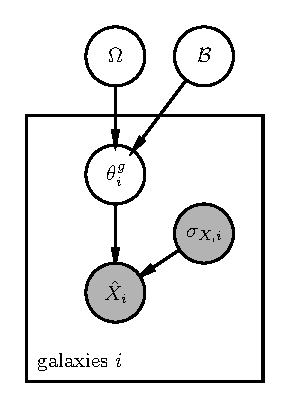
\includegraphics[width=0.4\textwidth]{figs/graph.pdf} 
    \caption{
        Graphical representation of our hierarchical approach that illustrate
        the relationship among the main parameters of our model. 
        Circles are inferred random variables, shaded circles are observed
        quantities, and dots indicate random variables that are deterministic.
    }\label{fig:graph}
\end{center}
\end{figure}


Given this hierarchical model, we can rewrite the posterior of interest: 
\begin{align}
p(\Omega, \mathcal{B} \given \{{\bfi X_i}\}) 
    =&~\frac{p(\Omega, \mathcal{B})~p(\{{\bfi X_i}\} \given \Omega, \mathcal{B})}{p(\{{\bfi X_i}\})}\\
    =&~\frac{p(\Omega, \mathcal{B})}{p(\{{\bfi X_i}\})}\int p(\{{\bfi X_i}\}
    \given \{\theta^g_i\})~p(\{\theta^g_i\} \given \Omega, \mathcal{B})~{\rm d}\{\theta^g_i\}.\\
    =&~\frac{p(\Omega, \mathcal{B})}{p(\{{\bfi X_i}\})}\prod\limits_{i=1}^N\int
    p({\bfi X_i} \given \theta^g_i)~p(\theta^g_i \given \Omega, \mathcal{B})~{\rm d}\theta^g_i\\
    =&~\frac{p(\Omega, \mathcal{B})}{p(\{{\bfi X_i}\})}\prod\limits_{i=1}^N\int
    \frac{p(\theta^g_i \given {\bfi X_i})~p({\bfi
    X_i})}{p(\theta^g_i)}~p(\theta^g_i \given \Omega, \mathcal{B})~{\rm d}\theta^g_i\\
    =&~p(\Omega, \mathcal{B})\prod\limits_{i=1}^N\int \frac{~p(\theta^g_i
    \given \Omega, \mathcal{B})}{p(\theta^g_i)} p(\theta^g_i \given {\bfi X_i})
    ~{\rm d}\theta^g_i\\
    =&~p(\Omega, \mathcal{B})\prod\limits_{i=1}^N\int \frac{p(\Omega, \mathcal{B}\given \theta^g_i)}{p(\Omega, \mathcal{B})}
p(\theta^g_i \given {\bfi X_i})~{\rm d}\theta^g_i \\
     \label{eq:post0}
    =&~\frac{1}{p(\Omega, \mathcal{B})^{N-1}}\prod\limits_{i=1}^N\int p(\Omega,
    \mathcal{B}\given \theta^g_i) p(\theta^g_i \given {\bfi X_i})~{\rm
    d}\theta^g_i  \\
     \label{eq:posterior}
    =&~\frac{1}{p(\Omega, \mathcal{B})^{N-1}}\prod\limits_{i=1}^N p(\Omega,
    \mathcal{B}\given {\bfi X_i}).
\end{align} 
With Eq.~\ref{eq:posterior}

explain that $\theta^g$ are latent variables. 


%\intertext{
%    We estimate the integral using $S_i$ Monte Carlo samples from the
%    individual posteriors $p(\theta^g_i \given {\bfi X_i})$: 
%}
%    \approx&~\frac{1}{p(\Omega, \mathcal{B})^{N-1}}\prod\limits_{i=1}^N\frac{1}{S_i}\sum\limits_{j=1}^{S_i} p(\Omega, \mathcal{B} \given \theta^g_{i,j}).

% --- discuss ---  
\input{discuss}
% --- summary ---  
\input{summary}

\section*{Acknowledgements}
It's a pleasure to thank

\appendix
\section{Validating the Neural Density Estimator} \label{sec:valid}
Our posterior (Eq.~\ref{eq:posterior}) requires an accurate estimate of the
individual posterior from NDE: 
$p(\Omega, \mathcal{B}\given {\bfi X_i}) \approx q_\phi(\Omega, \mathcal{B}\given {\bfi X_i})$
(Sec.~\ref{sec:anpe}). 
To validate $q_\phi$, we use 10\% of the CAMELS-TNG data reserved for testing
and two validation methods: (1) Simulation-Based Calilibration (SBC) and (2)
the ``distance to random point'' (DRP) coverage test. 

\begin{figure}[ht]
\vskip 0.2in
\begin{center}
    \centerline{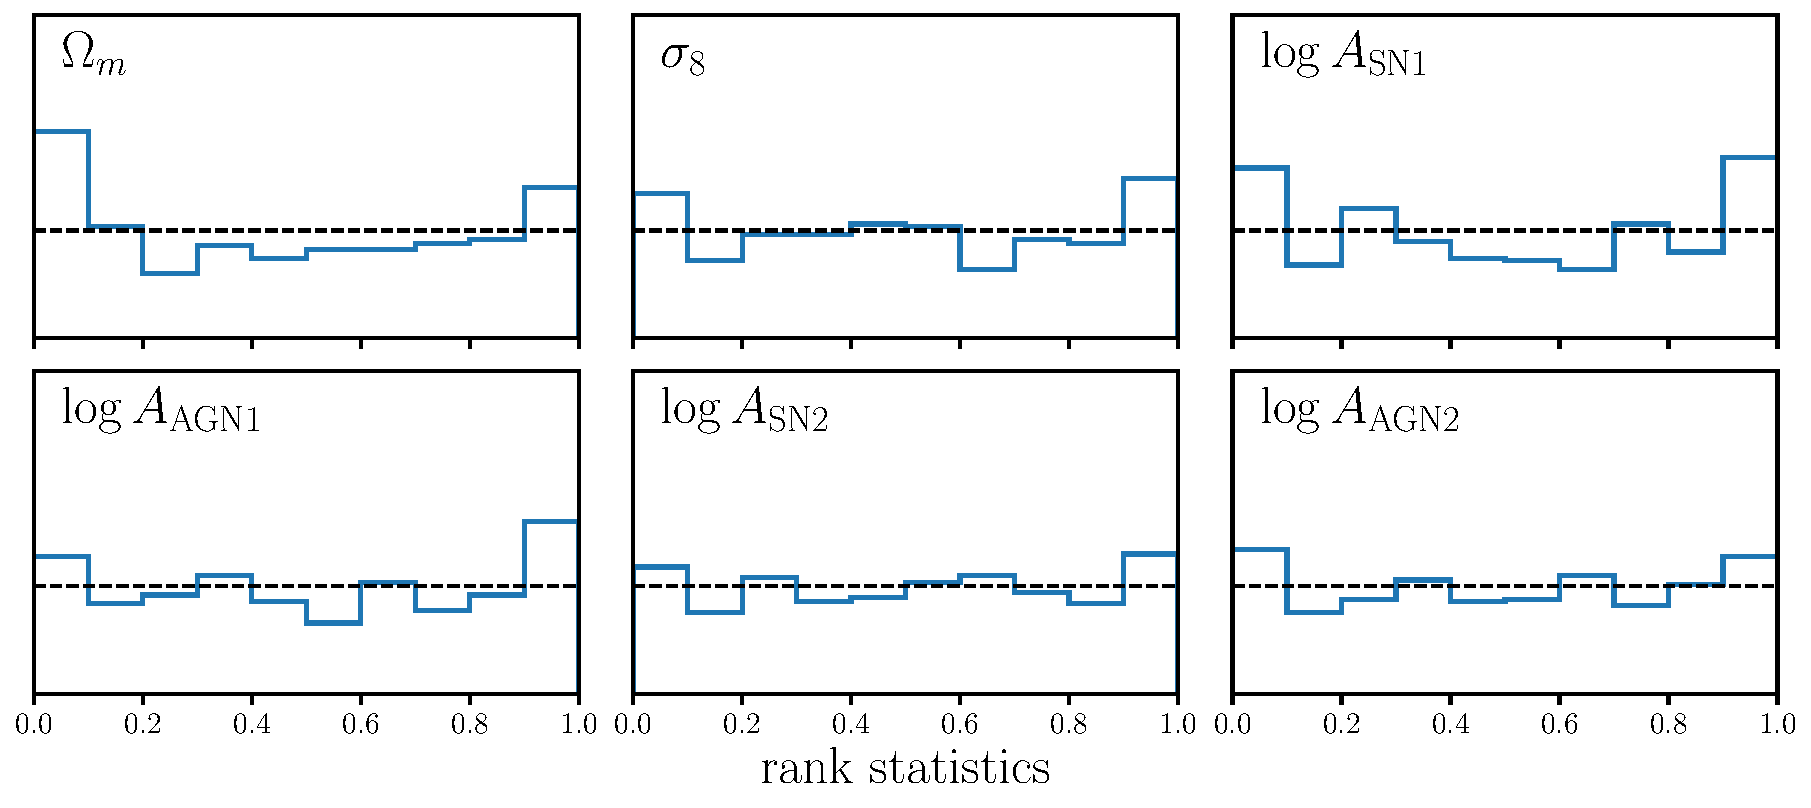
\includegraphics[width=0.9\columnwidth]{figs/ranks_p_omega_x.pdf}}
    \caption{
        Simulation-based calibration plot of 
        $q_\phi(\Omega, \mathcal{B}\given {\bfi X_i})$ using 10\% of the
        CAMELS-TNG data reserved for testing.
        The histogram in each panel represents the distribution of the rank
        statistic of the true value within the marginalized posterior (blue)
        for each parameter. 
        The rank distribution is uniform for the true posterior (black dashed).
        The rank distribution of $q_\phi$ is nearly uniform for all $\Omega$
        and $\mathcal{B}$ 
        parameters. 
        Therefore, it provides unbiased and accurate estimate of the true
        posterior.
    }\label{fig:ranks}
\end{center}
\vskip -0.2in
\end{figure}

Both are variations of the standard coverage test, where $q_\phi$ is applied to
test samples, not used for training. 
The posterior of each test sample is compared against the true parameter value
its percentile score is calculated.
Afterwards, cummulative distribution function (CDF) of the percentile is used
to access the accuracy of $q_\phi$.
SBC is a modification of this standard coverage test that uses rank statistics
rather than percentile score. 
It addresses the limitation that the CDFs only asymptotically approach the true
values and that the discrete sampling of the posterior can cause artifacts in
the CDFs. 
In Fig.~\ref{fig:ranks}, we present the SBC rank distributions of $q_\phi$ for
$\Omega$ and $\mathcal{B}$ (blue). 
For the true posterior, rank distribution is uniform by construction (black
dashed).
The rank distributions are nearly uniform for all $\Omega$ and
$\mathcal{B}$.
Hence, we confirm that $q_\phi$ is in excellent agreement with the true
posterior.


\begin{figure}[ht]
\vskip 0.2in
\begin{center}
    \centerline{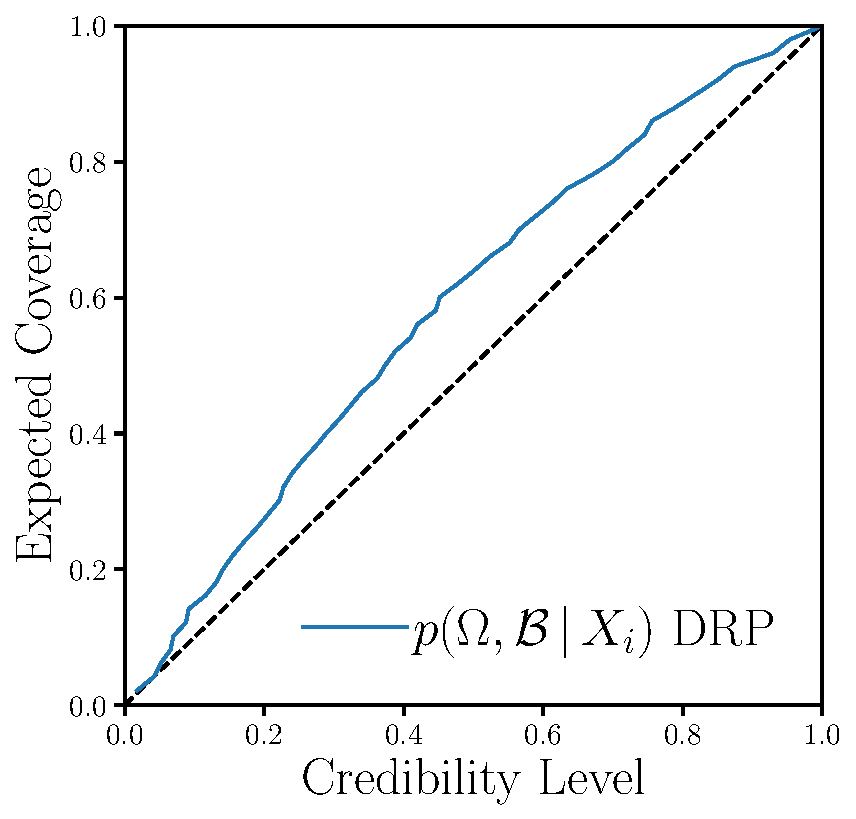
\includegraphics[width=0.4\columnwidth]{figs/tarp_p_omega_x.pdf}}
    \caption{DRP coverage test validating the accuracy of our 
    $q_{\phi}(\Omega, \mathcal{B}\given {\bfi X_i})$ posterior estimate (blue).
    The DRP test is calculated using  10\% of the CAMELS-TNG data reserved for
    testing.
    The black-dashed line represents an optimal estimate of the posterior.
    The DRP test demonstrates that $q_\phi$ provides a near optimal
    estimate of the true posterior.
    }\label{fig:tarp}
\end{center}
\vskip -0.2in
\end{figure}

As additional validation, we also use the DRP coverage test from
\cite{lemos2023}.
Instead of percentile scores or ranks, the DRP test assesses $q_\phi$ using
samples drawn from $q_\phi$ for a test sample, the true parameter value of the
test sample, and a random point in parameter space. 
It evalulates the distances between the $q_\phi$ samples and the random point. 
Then compares the distances to the distance between the true parameter value
and the random point in order to derive an estimate of expected coverage
probability. 
\cite{lemos2023} prove that this approach is necessary and sufficient to show
that a posterior estimator is optimal.
In Fig.~\ref{fig:tarp}, we present the DRP coverage test of $q_\phi$ (blue). 
Based ont he DRP test, $q_\phi$ provides a near optimal estimate of the
true posterior (black-dashed). 



\bibliographystyle{mnras}
\bibliography{cgpop} 
\end{document}
